\documentclass{beamer}

% For more themes, color themes and font themes, see:
% http://deic.uab.es/~iblanes/beamer_gallery/index_by_theme.html
%
\mode<presentation>
{
  \usetheme{Madrid}       % or try default, Darmstadt, Warsaw, ...
  \usecolortheme{crane} % or try albatross, beaver, crane, ...
  \usefonttheme{serif}    % or try default, structurebold, ...
  \setbeamertemplate{navigation symbols}{}
  \setbeamertemplate{caption}[numbered]
} 

\usepackage{tikz}
\usetikzlibrary{decorations.markings,angles}
\usepackage{tikz-3dplot} 

\usepackage{amsmath}


\begin{document}



\begin{frame}{FIRS FOV}

 
\begin{figure}[H]
 \centering
 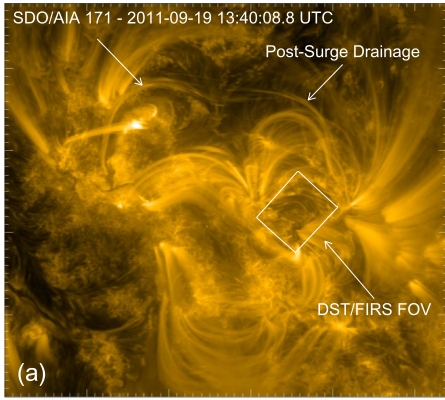
\includegraphics[scale=0.5]{img1.png}
%\caption{iron emission line at 600000K: upper transition region , quiet corona}
\end{figure}



\end{frame}

\begin{frame}{FIRS FOV}

 
\begin{figure}[H]
 \centering
 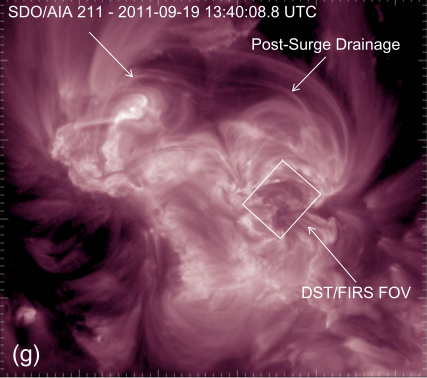
\includegraphics[scale=0.5]{img2.png}
%\caption{iron emission line at 2000000K: active regions conrona}
\end{figure}



\end{frame}
\begin{frame}{He velocity along loop}

 
\begin{figure}[H]
 \centering
 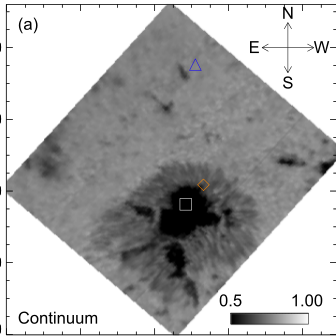
\includegraphics[scale=0.6]{sp_cont.png}
\end{figure}



\end{frame}





\begin{frame}{He velocity along loop}
 
\begin{figure}[H]
 \centering
 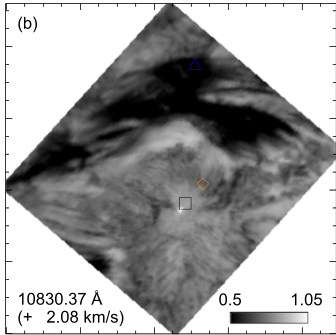
\includegraphics[scale=0.6]{spb.png}
\end{figure}

\end{frame}

\begin{frame}{He velocity along loop}
 
\begin{figure}[H]
 \centering
 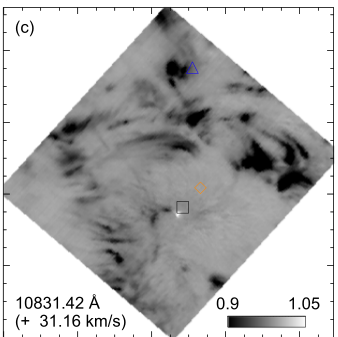
\includegraphics[scale=0.6]{spc.png}
\end{figure}

\end{frame}



\begin{frame}{He velocity along loop}
 
\begin{figure}[H]
 \centering
 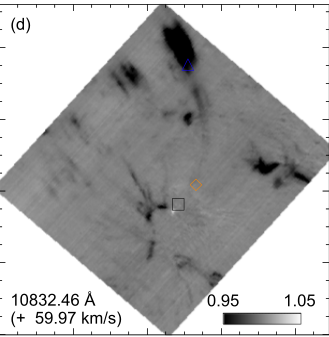
\includegraphics[scale=0.6]{spd.png}
\end{figure}

\end{frame}


\begin{frame}{He velocity along loop}
 
\begin{figure}[H]
 \centering
 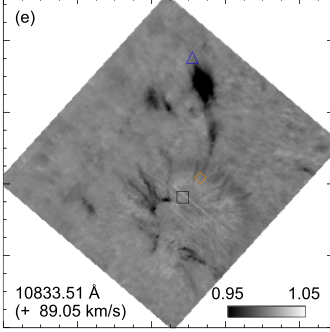
\includegraphics[scale=0.6]{spe.png}
\end{figure}

\end{frame}

\begin{frame}{He velocity along loop}
 
\begin{figure}[H]
 \centering
 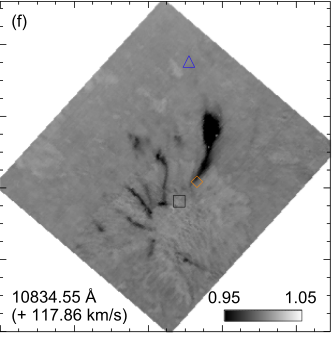
\includegraphics[scale=0.6]{spf.png}
\end{figure}

\end{frame}
\begin{frame}{He velocity along loop}
 
\begin{figure}[H]
 \centering
 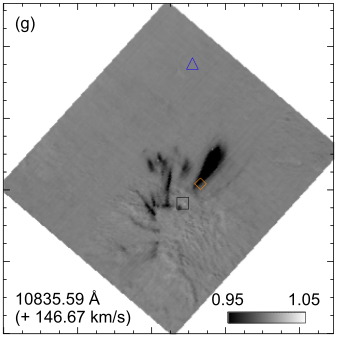
\includegraphics[scale=0.6]{spg.png}
\end{figure}

\end{frame}
\begin{frame}{He velocity along loop}
 
\begin{figure}[H]
 \centering
 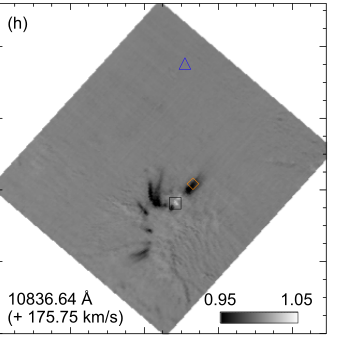
\includegraphics[scale=0.6]{sph.png}
\end{figure}

\end{frame}



\begin{frame}{He velocity along loop}

normalized to the local continuum intensity
 
\begin{figure}[H]
 \centering
 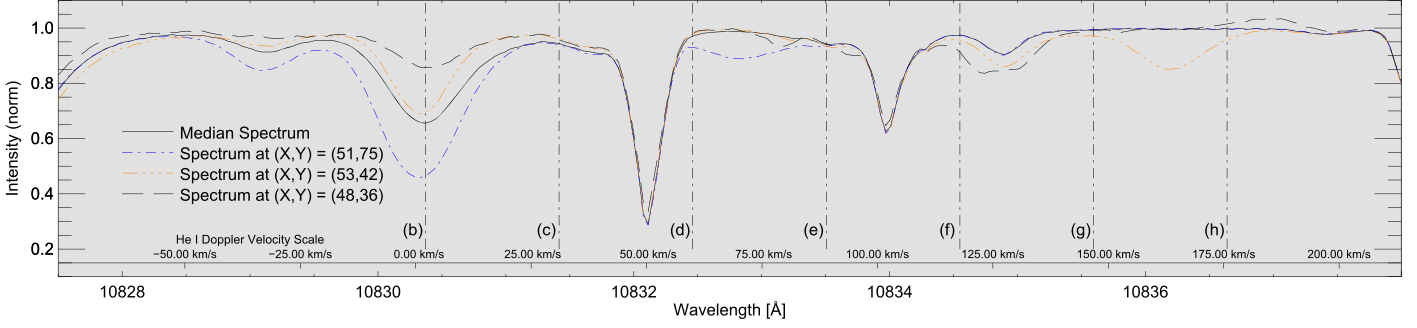
\includegraphics[scale=0.25]{sp_spec.png}
\caption{
spectral line profiles extracted from the
locations indicated in panels (a)–(h), illustrating the presence of additional He I velocity components redward of the telluric feature at 10832.1  \AA, and relative to the
median spectrum calculated using the entire data cube. An He I Doppler velocity scale bar is added for reference
}
\end{figure}



\end{frame}

\begin{frame}{Stereoscopic observations}

\begin{figure}[H]
 \centering
 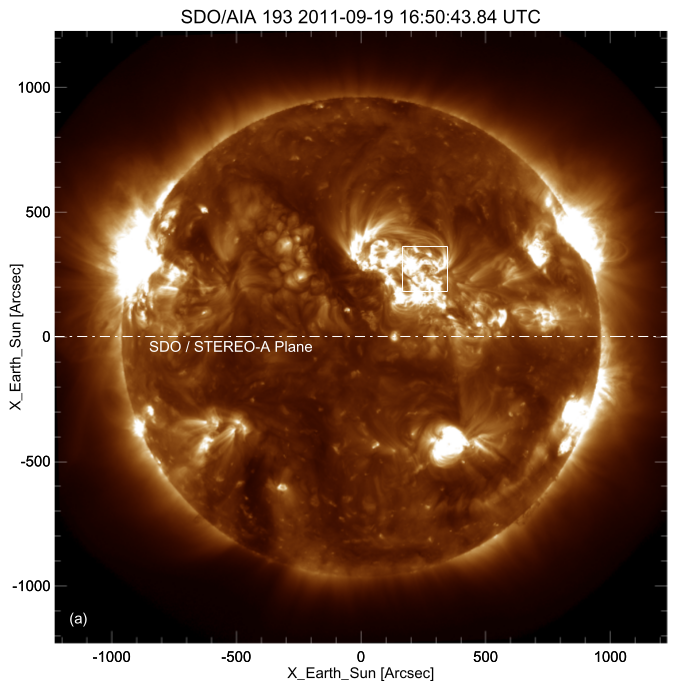
\includegraphics[scale=0.4]{sp_aia.png}
\end{figure}

\end{frame}
\begin{frame}{Stereoscopic observations}

\begin{figure}[H]
 \centering
 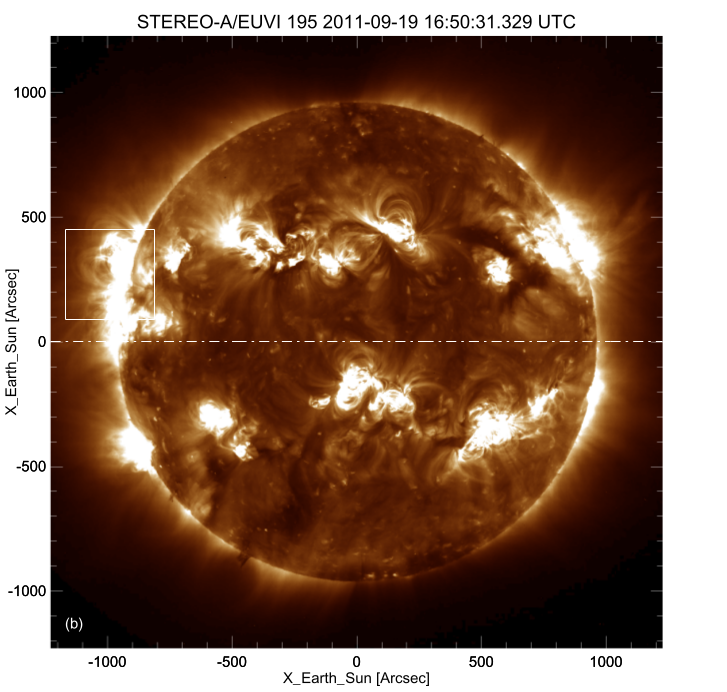
\includegraphics[scale=0.4]{sp_stereo.png}
\end{figure}

\end{frame}
\end{document}
